% Provenance (never printed): see sources/outline_sources.md (Year 2: monsoons; El Niño--Southern
% Oscillation; the North Atlantic Oscillation; ocean--atmosphere coupling). Definitions after the
% IPCC AR6 glossary, the NOAA CPC ENSO FAQ and NAO pages, the NWS glossary and the IMD monsoon
% FAQ; indices from the CPC data files (data/derived/bachelor-2-{oni,oni-table,roni,nino34,nao});
% figures from figdata/bachelor-2/climvar.py; values of the examples, exercises and problem
% computed in the Book 4 scratch calculator calc/ch23.py.
\chapter{التقلّب المناخي}\label{ch:b2:climate-variability}

في سبتمبر 2026 بلغ متوسط حرارة سطح البحر في وسط المحيط الهادئ الاستوائي \qty{29.27}{\celsius}،
حيث القيمة المعتادة لشهر سبتمبر \qty{26.71}{\celsius}؛ وأبعد شرقًا كانت أجزاء من المحيط
أدفأ من المعتاد بأكثر من \qty{4}{\celsius}، وقدّر المتنبّئون بأكثر من أربعة من خمسة
احتمال أن يتجاوز الحدث، بحلول نهاية السنة، كلّ \omterm{def:b2:climate-variability:enso}{إل نينيو} منذ عام 1950. وقد أدّت
الأحداث القياسية السابقة، في 1982 و1997 و2015، إلى ابيضاض المرجان وموته، وأشعلت الحرائق في الغابات المدارية
وجلبت موجات الحرّ؛ ويهبط صيد الأنشوفة في البيرو هبوطًا حادًّا حين يطول بقاء هذا الماء الدافئ. لقد
تأرجح المحيط والغلاف الجوي في المنطقة المدارية من الهادئ، كما يفعلان كلّ بضع سنوات، وامتدّ
التأرجح أبعد كثيرًا من المحيط الهادئ. يصف هذا
الفصل مثل هذه التأرجحات في المناخ، أي \omterm{def:b2:climate-variability:monsoon}{الرياح الموسمية}، \omterm{def:b2:climate-variability:enso}{وإل نينيو} \omterm{def:b2:climate-variability:enso}{ولا نينيا}، \omterm{def:b2:climate-variability:nao}{وتذبذب شمال
الأطلسي}، وما يجعل المحيط ذاكرتها.
% ledger: data:b4-nino34, cpc:edd-2026-10, thirumalai24:bjerknes, cheung26:peru

\begin{recall}
\textbf{من مجلّدات المدرسة}: الطقس والمناخ؛ وشذوذ درجة الحرارة؛ والطبقة المختلطة،
وطبقة التدرج الحراري والصعود؛ والتغذية الراجعة المناخية. \textbf{من مجلد السنة الأولى}: خلايا
هادلي، والرياح التجارية، ومنطقة التقارب بين المدارين وهجرتها الفصلية، ودورة
واكر، والصعود الساحلي. \textbf{من \cref{ch:b2:weather-systems}}: التيّار النفّاث،
وأمواج روسبي، والأعاصير خارج المدارية \omterm{def:b2:weather-systems:blocking}{والحجب الجوّي}. \textbf{من كتب الفيزياء}: السعة الحرارية
والقانون الأول للديناميكا الحرارية.
\end{recall}

\section{التقلّب ومقاييسه}\label{sec:b2:climate-variability:measures}

يتغيّر الطقس من يوم إلى يوم؛ والمناخ، أي إحصاءات الطقس، يتغيّر هو أيضًا، من فصل
أو سنة إلى التالية، حتى حين لا يتغيّر شيء خارج النظام المناخي. وبعض ذلك
التقلّب ضجيج، لكن كثيرًا منه منتظم في أنماط قليلة تتكرّر، لكلّ منها
جغرافيتها ومقاييسها الزمنية.

\begin{definition}[نمط التقلّب المناخي؛ المؤشّر المناخي؛ المعدّل المناخي]\label{def:b2:climate-variability:modes}
\emph{نمط التقلّب المناخي}\index{نمط التقلّب المناخي} نمط متكرّر من
التقلّب الطبيعي للنظام المناخي، له توزّعه المكاني وفصليته ومقاييسه
الزمنية، ينشأ من ديناميكا الغلاف الجوي أو من اقتران المحيط
بالغلاف الجوي. و\emph{المؤشّر المناخي}\index{المؤشّر المناخي} سلسلة زمنية مبنية من متغيّرات
مناخية تلخّص حالة مثل هذا النمط، ومثاله فرق ضغط مستوى
سطح البحر بين آيسلندا والأزور. و\emph{المعدّل المناخي}\index{المعدّل المناخي} لمتغيّر
هو متوسطه على فترة مرجعية، يُحسب لكلّ شهر تقويمي أو فصل؛ وطول الفترة
المرجعية القياسية 30 سنة، وهي حاليًّا 1991--2020.
\end{definition}
% ledger: ipccgl:modes, ipccgl:index, wmo:normal-30yr

كثير من الأنماط تحرّكه عمليات داخلية في النظام المناخي: فهي جزء من
تقلّبه الداخلي. ولأنها تتكرّر بمقاييسها الزمنية الخاصة، فهي مصدر
لقابلية التنبّؤ أبعد من مدى تنبّؤات الطقس، من أسابيع إلى عقود. والمؤشّرات تجعلها
قابلة للقياس. ويُحسب المؤشّر من حالات الشذوذ، كما في مجلّدات المدرسة، ثم
يُملَّس.
% ledger: ipccgl:modes

\begin{method}[من الأرصاد إلى مؤشّر]\label{met:b2:climate-variability:index}
\begin{enumerate}
  \item احسب \omterm{def:b2:climate-variability:modes}{المعدّل المناخي}: متوسط المتغيّر لكلّ شهر تقويمي على امتداد
        الفترة المرجعية.
  \item اطرحه: شذوذ كلّ شهر هو قيمته مطروحًا منها \omterm{def:b2:climate-variability:modes}{المعدّل المناخي} لذلك الشهر.
        فتختفي الدورة الفصلية؛ وما يبقى هو التقلّب.
  \item ملِّس حالات الشذوذ بمتوسط متحرّك، أي متوسط $n$ قيمة متتالية متمركزة على
        كلّ شهر، لإزالة التذبذبات الأقصر من النمط المدروس.
  \item إذا كان المؤشّر سيُقارن بغيره، فاقسمه على انحرافه المعياري: فيصبح المؤشّر
        معياريًّا، بوحدات الانحراف المعياري.
\end{enumerate}
\end{method}

\begin{example}[شذوذ]\label{ex:b2:climate-variability:anomaly}
بلغ متوسط حرارة سطح البحر في وسط المحيط الهادئ الاستوائي بين \ang{5} شمالًا
و\ang{5} جنوبًا، و\ang{170} غربًا و\ang{120} غربًا، \qty{29.27}{\celsius} في سبتمبر 2026. ومعدّله المناخي
لشهر سبتمبر \qty{26.71}{\celsius}، فكان الشذوذ $29.27 - 26.71 = \qty{2.56}{\celsius}$.
وفي سبتمبر 1997 كان المحيط نفسه عند \qty{28.79}{\celsius} مقابل \qty{26.73}{\celsius}، أي
شذوذ قدره \qty{2.06}{\celsius}. ويختلف المعدّلان المناخيان قليلًا لأن الفترة المرجعية
تُزاح كلّ خمس سنوات: فالمحيط نفسه قد ازداد دفئًا.
% ledger: data:b4-nino34, cpc:oni-def
\end{example}

\section{الرياح الموسمية}\label{sec:b2:climate-variability:monsoons}

\begin{definition}[الرياح الموسمية]\label{def:b2:climate-variability:monsoon}
\emph{الرياح الموسمية}\index{الرياح الموسمية} ريح حرارية المنشأ، تنشأ من اختلاف تسخين
كتلة يابسة والمحيط المجاور لها، ينعكس اتجاهها مع الفصول، مع ما تجلبه
من انعكاس فصلي في الهطول.
\end{definition}
% ledger: nws4:monsoon, ipccgl:monsoon

على اليابسة تبقى حرارة شمس الصيف في طبقة رقيقة قرب السطح، بينما يمزج البحر
الحرارة نفسها نزولًا عبر طبقته المختلطة، التي يبلغ عمقها عشرات الأمتار، فيسخن أقلّ بكثير. فالهواء فوق
اليابسة يسخن أكثر، فينخفض ضغطه عند السطح، ويتدفّق هواء رطب من البحر، فيصعد ويبرد
ويمطر؛ وفي الأعالي يعود الهواء نحو البحر. وفي الشتاء تكون اليابسة السطح الأبرد فتنعكس
الدورة. ومجتمعةً، تكوّن \omterm{def:b2:climate-variability:monsoon}{الرياح الموسمية} في الكوكب نمطًا عالميًّا واحدًا يهيمن على الدورة
السنوية للأمطار المدارية وشبه المدارية؛ ويُعرَّف نطاقه بأنه المناطق التي يتجاوز فيها متوسط مطر
الصيف المحلّي مطر الشتاء بأكثر من \qty{2.5}{mm} في اليوم.
% ledger: nws4:monsoon, ipccgl:monsoon

\begin{omfigure}
\centering
\begin{tikzpicture}[font=\scriptsize, >=Stealth]
\foreach \col/\title in {0/{أ\enspace الصيف}, 7.2/{ب\enspace الشتاء}} {
  \begin{scope}[shift={(\col,0)}]
  \node[anchor=south west] at (0,3.0) {\textbf{\title}};
  \fill[ocBlue!18] (0,0) rectangle (3,0.35);
  \fill[brown!35] (3,0) -- (6.4,0) -- (6.4,0.5) -- (3,0.35) -- cycle;
  \node at (1.5,0.17) {بحر};
  \node at (4.7,0.2) {يابسة};
  \end{scope}
}
% summer: low over the land, inflow from the sea, rising air and rain
\node[font=\small\bfseries, ocBlue] at (0.45,0.62) {ع};
\node[font=\small\bfseries, ocRed] at (4.8,0.78) {م};
\node[ocRed, anchor=west] at (5.35,0.78) {حارّ};
\draw[->, thick] (1.0,0.98) -- (4.2,1.02);
\node at (2.4,0.66) {هواء رطب من البحر};
\draw[->, thick] (4.8,1.15) -- (4.8,2.55);
\draw[->, thick] (4.45,2.8) -- (1.75,2.8);
\draw[->, thick] (1.4,2.6) -- (1.4,1.25);
\fill[black!15, draw=black!40] (4.0,1.9) .. controls (4.0,2.55) and (5.6,2.55) .. (5.6,1.9) -- cycle;
\foreach \x in {4.25,4.5,5.1,5.35} {\draw[ocBlue, dashed] (\x,1.85) -- (\x-0.1,1.2);}
\node[anchor=west] at (5.65,2.1) {مطر};
% winter: high over the land, dry outflow to the sea
\begin{scope}[shift={(7.2,0)}]
\node[font=\small\bfseries, ocRed] at (0.45,0.62) {م};
\node[font=\small\bfseries, ocBlue] at (4.8,0.78) {ع};
\node[ocBlue, anchor=west] at (5.35,0.78) {بارد};
\draw[->, thick] (4.2,1.02) -- (1.0,0.98);
\node at (2.4,0.66) {هواء جاف من اليابسة};
\draw[->, thick] (1.4,1.25) -- (1.4,2.6);
\draw[->, thick] (1.75,2.8) -- (4.45,2.8);
\draw[->, thick] (4.8,2.55) -- (4.8,1.15);
\end{scope}
\end{tikzpicture}
\par\smallskip{\small \omterm{def:b2:climate-variability:monsoon}{الرياح الموسمية} دورةً بين اليابسة والبحر (مقطع تخطيطي، ليس على مقياس الرسم): في
الصيف تكون اليابسة السطح الأدفأ، مع ضغط منخفض عند الأرض (م)، وتدفّق هواء رطب من
البحر، وهواء صاعد ومطر؛ وفي الشتاء تنعكس الدورة وتكون ريح اليابسة جافّة (ع: مرتفع).}
\end{omfigure}
% ledger: nws4:monsoon, imd:heat-low

تبدأ \omterm{def:b2:climate-variability:monsoon}{الرياح الموسمية} لجنوب آسيا وجنوب شرقها في أواخر مايو أو أوائل يونيو، وتتقدّم
نحو الشمال الشرقي وتنتهي في أواخر سبتمبر أو أوائل أكتوبر. وقبلها تسخن الأراضي المحيطة
ببحر العرب: ففي يونيو يرسل السطح نحو \qty{160}{W/m^2} من الحرارة إلى الهواء فوق
الشمال الغربي الجافّ من الهند وباكستان والشرق الأوسط، فيتكوّن هناك منخفض حراري ضحل،
لا يتجاوز ارتفاعه نحو \qty{1.5}{km}، قليل المطر؛ والمنخفض الحراري الضعيف، كما في سنة الجفاف
1987، يعني جذبًا ضعيفًا لهواء المحيط الرطب. ومنه يمتدّ أخدود مستطيل من الضغط المنخفض، هو أخدود
\omterm{def:b2:climate-variability:monsoon}{الرياح الموسمية}، إلى رأس خليج البنغال؛ وتذبذباته بين الشمال والجنوب تجلب فترات
النشاط وفترات الانقطاع في الموسم. وعلى الهند كلّها يبلغ متوسط مطر يونيو إلى سبتمبر
\qty{88}{cm}، بانحراف معياري قدره \qty{9}{cm}، أي نحو \qty{10}{\percent}: ويُسمّى الموسم الذي يبقى ضمن
\qty{10}{\percent} من متوسط الفترة الطويلة عاديًّا. وعلى ساحل كيرالا، حيث تعلن
مصلحة الأرصاد الوطنية بدء \omterm{def:b2:climate-variability:monsoon}{الرياح الموسمية} انطلاقًا من أمطار أربع عشرة محطّة،
والرياح والأشعة تحت الحمراء الصادرة المقيسة بالأقمار الصناعية، يبلغ متوسط المطر
\qty{556}{mm} في يونيو و\qty{659}{mm} في يوليو.
% ledger: ipccgl:monsoon, imd:heat-low, imd:lpa, imd:onset

تجلب \omterm{def:b2:climate-variability:monsoon}{الرياح الموسمية} لغرب أفريقيا رياحًا جنوبية غربية رطبة من خليج غينيا، تتقدّم
شمالًا من مايو إلى سبتمبر؛ ويبلغ مطرها ذروته قرب \ang{12} شمالًا في أواخر أغسطس وفي سبتمبر
ويتراجع ابتداءً من أكتوبر.
% ledger: ipccgl:monsoon

\omterm{def:b2:climate-variability:monsoon}{الرياح الموسمية} منتظمة في توقيتها، غير منتظمة في كمّيتها، وتأرجحات المحيط الهادئ المداري
من سنة إلى أخرى من أسباب ذلك. فسنوات \omterm{def:b2:climate-variability:enso}{إل نينيو} تميل إلى ترك الهند في نقص من المطر:
فقد جاءت موجات الجفاف في 1904 و1972 و1987 مع \omterm{def:b2:climate-variability:enso}{إل نينيو}. والصلة ليست أكيدة: ففي 1997 تزامن
\omterm{def:b2:climate-variability:enso}{إل نينيو} قويّ مع طور موجب لثنائي القطب في المحيط الهندي، وهو نمط نلقاه أدناه، وشهدت الهند
موسمًا قريبًا من العادي.
% ledger: narang24:enso-monsoon, ipccgl:other-modes

\section{إل نينيو والتذبذب الجنوبي}\label{sec:b2:climate-variability:enso}

وصف مجلد السنة الأولى دورة واكر: هواء يصعد فوق غرب المحيط الهادئ الدافئ،
ويتدفّق شرقًا في الأعالي، ويهبط فوق شرق المحيط الهادئ البارد ويعود غربًا مع الرياح
التجارية. وفي المحيط تحته، تكدّس الرياح التجارية الماء الدافئ في الغرب، حيث تكون طبقة التدرج الحراري
عميقة، وتسحب الماء البارد إلى الأعلى على امتداد خطّ الاستواء في الشرق، حيث تكون ضحلة. وهذه الحالة ليست
ثابتة.

\begin{definition}[إل نينيو--التذبذب الجنوبي؛ إل نينيو؛ لا نينيا؛ التذبذب الجنوبي]\label{def:b2:climate-variability:enso}
\emph{إل نينيو--التذبذب الجنوبي}\index{إل نينيو--التذبذب الجنوبي} (ENSO) هو
النمط المقترن بين المحيط والغلاف الجوي في المحيط الهادئ المداري: تغيّرات متّسقة من سنة إلى أخرى في
حرارة سطح البحر، والمطر الحملي، والضغط السطحي والدورة على امتداد
المحيط الهادئ الاستوائي، بمقاييس زمنية مفضّلة من سنتين إلى نحو سبع سنوات. و\emph{إل
نينيو}\index{إل نينيو} طوره الدافئ، أي احترار سطح البحر في وسط المحيط الهادئ الاستوائي
ووسطه الشرقي؛ و\emph{لا نينيا}\index{لا نينيا} طوره البارد، أي تبرّد
المنطقة نفسها. و\emph{التذبذب الجنوبي}\index{التذبذب الجنوبي} جزؤه الجوّي،
أي أرجحة في الضغط السطحي بين غرب المحيط الهادئ المداري وشرقه: ففي أثناء إل نينيو
يكون الضغط أعلى من المتوسط فوق إندونيسيا وغرب المحيط الهادئ وأدنى فوق
شرقه، والعكس في أثناء لا نينيا.
\end{definition}
% ledger: cpc:enso-faq, cpc:enso-faq-so, ipccgl:enso

في أثناء \omterm{def:b2:climate-variability:enso}{إل نينيو} تضعف الرياح التجارية الشرقية على امتداد خطّ الاستواء، وفي الغرب قد
تهبّ الرياح القريبة من السطح حتى من الغرب؛ وينتشر الماء الدافئ في الغرب نحو الشرق، ويتبعه الحمل
العميق ومطره، تاركًا إندونيسيا وشمال أستراليا أجفّ. ويكون سطح البحر
في وسط المحيط الهادئ الشرقي عادةً أدفأ من المتوسط بمقدار \qtyrange{1.5}{2.5}{\celsius}، وتقع
طبقة التدرج الحراري هناك على عمق \qtyrange{150}{175}{m}، أعمق من المعتاد. وفي أثناء \omterm{def:b2:climate-variability:enso}{لا نينيا} تقوى الرياح
التجارية عبر الحوض كلّه، ويكون سطح البحر أبرد من المتوسط بمقدار \qtyrange{1}{2}{\celsius}،
وترتفع طبقة التدرج الحراري في الشرق إلى \qtyrange{50}{100}{m}. وتضعف دورة واكر
في أثناء \omterm{def:b2:climate-variability:enso}{إل نينيو} وتقوى في أثناء \omterm{def:b2:climate-variability:enso}{لا نينيا}. وتتكرّر النوبات عادةً كلّ ثلاث إلى
خمس سنوات، بفواصل تراوحت بين سنتين وسبع؛ ويدوم \omterm{def:b2:climate-variability:enso}{إل نينيو} عادةً تسعة إلى
اثني عشر شهرًا، \omterm{def:b2:climate-variability:enso}{ولا نينيا} سنة إلى ثلاث سنوات. ويميل كلاهما إلى النشوء بين مارس ويونيو،
وإلى بلوغ الذروة بين ديسمبر وأبريل وإلى الضعف بين مايو ويوليو؛ وتكون آثارهما أشدّ
من ديسمبر إلى أبريل، حين يكون سطح البحر الاستوائي في أدفأ حالاته.
% ledger: cpc:enso-faq-features, cpc:enso-faq-timing

\begin{omfigure}
\centering
\begin{tikzpicture}[font=\scriptsize, >=Stealth, x=1cm, y=0.8cm]
\foreach \row/\title/\tw/\te/\rx/\cwidth in {
    0/{أ\enspace محايد}/1.15/0.35/1.6/1.0,
    -4.6/{ب\enspace إل نينيو}/0.95/0.85/5.6/1.4,
    -9.2/{ج\enspace لا نينيا}/1.3/0.18/1.0/0.8} {
  \begin{scope}[shift={(0,\row)}]
  \node[anchor=south west] at (0,2.55) {\textbf{\title}};
  % ocean: warm layer above the thermocline
  \fill[ocBlue!20] (0,-1.5) rectangle (11,0);
  \fill[omWarm!25] (0,0) -- (0,-\tw) .. controls (4,-\tw) and (7,-\te) .. (11,-\te) -- (11,0) -- cycle;
  \draw[thick, ocBlue!70!black] (0,-\tw) .. controls (4,-\tw) and (7,-\te) .. (11,-\te);
  \draw (0,0) -- (11,0);
  % convection and Walker cell
  \fill[black!15, draw=black!40] ({\rx-\cwidth/2},0.5) .. controls ({\rx-\cwidth/2},2.1) and ({\rx+\cwidth/2},2.1) .. ({\rx+\cwidth/2},0.5) -- cycle;
  \draw[->, thick] (\rx,0.55) -- (\rx,2.15);
  \draw[->, thick] ({\rx+0.4},2.3) -- (9.6,2.3);
  \draw[->, thick] (10.0,2.1) -- (10.0,0.5);
  \draw[->, thick] (9.6,0.3) -- ({\rx+0.7},0.3);
  \end{scope}
}
\node[anchor=west] at (2.3,1.4) {هواء صاعد، مطر};
\node[anchor=east] at (9.9,1.4) {هواء هابط};
\node at (6.0,0.55) {رياح تجارية};
\node[anchor=west, ocBlue!70!black] at (7.6,-0.95) {طبقة التدرج الحراري};
\node[anchor=east] at (4.8,-4.6+1.4) {المطر ينتقل شرقًا};
\node at (8.2,-4.6+0.55) {رياح تجارية ضعيفة};
\node at (6.0,-9.2+0.55) {رياح تجارية قويّة};
\node[ocBlue!70!black, align=center] at (9.6,-9.2-0.8) {ماء بارد\\قرب السطح};
\node[anchor=north west] at (0,-9.2-1.55) {\foreignlanguage{arabic}{الغرب (إندونيسيا)}};
\node[anchor=north east] at (11,-9.2-1.55) {\foreignlanguage{arabic}{الشرق (أمريكا الجنوبية)}};
\end{tikzpicture}
\par\smallskip{\small المحيط الهادئ الاستوائي على امتداد خطّ الاستواء في أطوار ENSO الثلاثة
(تخطيطي، ليس على مقياس الرسم): دورة واكر في الأعلى، والطبقة العليا الدافئة
وطبقة التدرج الحراري في الأسفل. في أثناء \omterm{def:b2:climate-variability:enso}{إل نينيو} تضعف الرياح التجارية، وينتشر الماء الدافئ والمطر شرقًا
وتتعمّق طبقة التدرج الحراري في الشرق إلى \qtyrange{150}{175}{m}؛ وفي أثناء \omterm{def:b2:climate-variability:enso}{لا نينيا} تقوى الرياح التجارية
وترتفع طبقة التدرج الحراري في الشرق إلى \qtyrange{50}{100}{m}.}
\end{omfigure}
% ledger: cpc:enso-faq-features, climategov:walker

جاءت الأسماء من قرون مختلفة ومن علوم مختلفة. فقد لاحظ صيّادو ساحل
أمريكا الجنوبية احترارًا لمياههم الساحلية حول عيد الميلاد يربك
الصيد، فسمّوه \omterm{def:b2:climate-variability:enso}{إل نينيو}، أي الطفل الصبي. واكتشف السير غيلبرت واكر \omterm{def:b2:climate-variability:enso}{التذبذب
الجنوبي} في الغلاف الجوي، دون أن يربطه بالمحيط. ولم يرَ ياكوب بيركنس وآخرون إلا في أواخر ستينيات القرن العشرين أن
الاثنين ظاهرة واحدة. واكتسب مصطلحا \omterm{def:b2:climate-variability:enso}{لا نينيا} والمحايد شهرتهما في ثمانينيات القرن العشرين.
% ledger: climategov:enso-history, ipccgl:enso

\begin{history}[الطفل الصبي عند الصيّادين]
\begin{minipage}[t]{0.54\linewidth}\vspace{0pt}
قبالة ساحل البيرو الجافّ، يكون الماء البارد الذي تسحبه الرياح إلى الأعلى على امتداد الشاطئ غنيًّا
بالمغذّيات ويغذّي مصايد منتجة. وقد عرف صيّادوه احترارًا يأتي حول
عيد الميلاد، حين يندر السمك، فأعطوه اسم طفل الموسم. ولا يزال
صيد الأنشوفة في البيرو يتبع ENSO: ففي تحليل حديث، جعلت حالات الشذوذ الحراري المرتفع المطوّلة
صيدًا منخفضًا جدًّا أرجح بأكثر من تسع مرّات، مع هبوط وسيط في
الصيد بنحو \qty{60}{\percent}؛ ويبرز \omterm{def:b2:climate-variability:enso}{إل نينيو} القويّ في 1997--98 في السجلّ.
\end{minipage}\hfill
\begin{minipage}[t]{0.42\linewidth}\vspace{0pt}
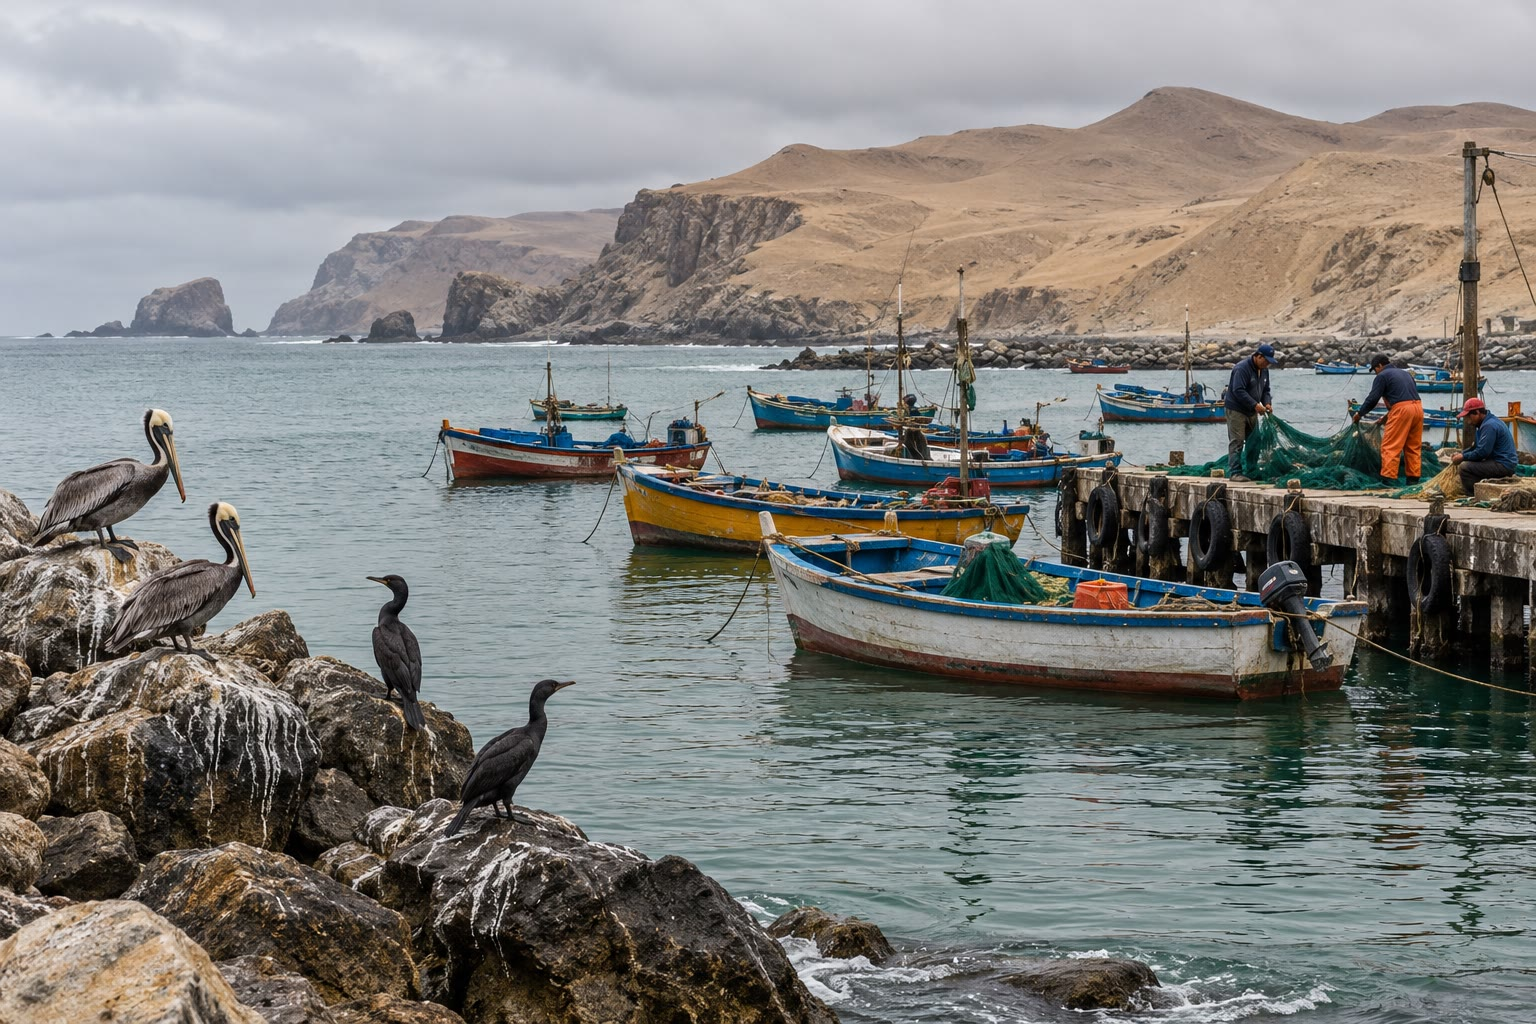
\includegraphics[width=\linewidth]{images/book4/ai/b2-fishing-harbour.jpg}

{\scriptsize قوارب صيد في ميناء على ساحل صحراوي مياهه الصاعدة باردة
(رسم توضيحي مولَّد بالذكاء الاصطناعي).}
\end{minipage}
% ledger: climategov:enso-history, cheung26:peru, stewart:upwelling
\end{history}

لماذا يتأرجح النظام أصلًا؟ لأن المحيط والغلاف الجوي في المنطقة الاستوائية من الهادئ
يعزّز كلّ منهما حالات شذوذ الآخر.

\begin{definition}[التغذية الراجعة لبيركنس]\label{def:b2:climate-variability:bjerknes}
\emph{التغذية الراجعة لبيركنس}\index{التغذية الراجعة لبيركنس} هي التغذية الراجعة الموجبة بين
حرارة سطح البحر والرياح والتيّارات المحيطية في المحيط الهادئ الاستوائي: فاحترار
الشرق يُضعف فرق الحرارة والضغط بين الشرق والغرب، ومن ثَمّ الرياح التجارية؛
والرياح التجارية الأضعف تدع الماء الدافئ في الغرب ينتشر شرقًا وتصعد بماء بارد أقلّ في
الشرق، فيزداد الشرق احترارًا. والحلقة نفسها تضخّم التبرّد.
\end{definition}
% ledger: thirumalai24:bjerknes, cpc:enso-faq-timing

\begin{omfigure}
\centering
\begin{tikzpicture}[font=\small, >=Stealth, box/.style={draw, rounded corners=2pt, fill=omDef!8,
  align=center, text width=4.3cm, minimum height=1.05cm, inner sep=3pt}]
\node[box] (a) at (0,2) {شرق المحيط الهادئ الاستوائي\\أدفأ من المعتاد};
\node[box] (b) at (6.2,2) {فرق أصغر بين الشرق والغرب\\في الحرارة والضغط};
\node[box] (c) at (6.2,0) {رياح تجارية أضعف};
\node[box] (d) at (0,0) {الماء الدافئ ينتشر شرقًا،\\والماء البارد الصاعد أقلّ};
\draw[->, very thick, ocRed] (a) -- (b);
\draw[->, very thick, ocRed] (b) -- (c);
\draw[->, very thick, ocRed] (c) -- (d);
\draw[->, very thick, ocRed] (d) -- (a);
\node[ocRed, font=\bfseries] at (3.1,1) {$+$};
\end{tikzpicture}
\par\smallskip{\small \omterm{def:b2:climate-variability:bjerknes}{التغذية الراجعة لبيركنس}، مرسومة لحالة احترار؛ وإذا عُكس كلّ سهم، فإن
الحلقة نفسها تعمّق التبرّد. والحلقة الموجبة من هذا النوع تضخّم الاضطراب الصغير.}
\end{omfigure}
% ledger: thirumalai24:bjerknes

التغذية الراجعة الموجبة تفسّر كيف ينمو الشذوذ، لا كيف يبدأ أو ينتهي. ففي أحد التفسيرات الحالية،
يبدأ \omterm{def:b2:climate-variability:enso}{إل نينيو} حين تُضعف تذبذبات عشوائية في الرياح التجارية التيّارات الاستوائية التي
تُبقي الماء الدافئ في الغرب؛ فينتشر الحوض الدافئ شرقًا، ويتبعه الحمل،
وتتولّى \omterm{def:b2:climate-variability:bjerknes}{التغذية الراجعة لبيركنس} الأمر فينمو الحدث. أمّا أحداث \omterm{def:b2:climate-variability:enso}{لا نينيا}، في التفسير نفسه، فيطلقها
\omterm{def:b2:climate-variability:enso}{إل نينيو} سابق. وأبسط النماذج التي تجعل النظام يتذبذب، ومنها نموذج مذبذب
إعادة الشحن، تقرن بين كمّيتين: شذوذ حرارة سطح البحر في وسط
المحيط الهادئ وحجم الماء الدافئ في أعلى المحيط المختزن على امتداد خطّ الاستواء. فشذوذ الحرارة
يفرّغ ذلك المخزون أو يعيد ملأه عبر الرياح التي يحرّكها، والمخزون، عبر
عمق طبقة التدرج الحراري، يهيّئ الطور التالي. ويحلّ \cref{exo:b2:climate-variability:10}
زوجًا كهذا من المعادلات.
% ledger: thirumalai24:bjerknes, stuecker25:ro

لتتبّع ENSO، تستعمل مراكز الرصد مؤشّرات.

\begin{definition}[مؤشّر نينيو-3.4؛ المؤشّر المحيطي لإل نينيو]\label{def:b2:climate-variability:oni}
\emph{مؤشّر نينيو-3.4}\index{مؤشّر نينيو-3.4} هو الشذوذ الشهري لحرارة سطح
البحر متوسَّطةً على المنطقة \ang{5} شمالًا--\ang{5} جنوبًا، \ang{170} غربًا--\ang{120} غربًا، بالنسبة إلى
\omterm{def:b2:climate-variability:modes}{المعدّل المناخي} لفترة أساس طولها 30 سنة متمركزة على السنة، تُحدَّث كلّ خمس سنوات.
و\emph{المؤشّر المحيطي لإل نينيو}\index{المؤشّر المحيطي لإل نينيو} (ONI) هو متوسطه المتحرّك على ثلاثة أشهر. ونوبة
\omterm{def:b2:climate-variability:enso}{إل نينيو} (أو \omterm{def:b2:climate-variability:enso}{لا نينيا}) هي تتابع من خمسة فصول ثلاثية الأشهر متداخلة متتالية على الأقلّ
يكون فيها المؤشّر ONI عند \qty{+0.5}{\celsius} أو فوقها (عند \qty{-0.5}{\celsius} أو دونها).
\end{definition}
% ledger: cpc:oni-def, cpc:enso-faq

الفصول متداخلة: DJF وJFM وFMA وهكذا، كلّ منها متوسط ثلاثة أشهر، ويشترك كلّ منها في شهرين
مع الذي يليه. ومؤشّر ثانٍ، هو مؤشّر \omterm{def:b2:climate-variability:enso}{التذبذب الجنوبي}، يتتبّع الغلاف الجوي: فهو
يُحسب من انحرافات فرق الضغط بين تاهيتي وداروين، ويكون سالبًا
في أثناء \omterm{def:b2:climate-variability:enso}{إل نينيو}، وموجبًا في أثناء \omterm{def:b2:climate-variability:enso}{لا نينيا}. ومنذ فبراير 2026 صار المؤشّر الرسمي لرصد
ENSO مؤشّرًا ONI نسبيًّا، يُحسب من شذوذ نينيو-3.4 مطروحًا منه متوسط شذوذ المحيط
المداري كلّه بين \ang{20} شمالًا و\ang{20} جنوبًا، ثم يُعاد تقييسه إلى سعة المؤشّر ONI. ولأنه
يُقاس بالنسبة إلى المنطقة المدارية كلّها، فهو أقلّ تأثّرًا باختيار فترة الأساس بينما تزداد المحيطات
دفئًا، وهو أوثق صلة بأمطار المحيط الهادئ المداري. وفي سبتمبر 2026 كان
الشذوذ النسبي لمنطقة نينيو-3.4 \qty{2.08}{\celsius}، مقابل \qty{2.56}{\celsius}
في \cref{ex:b2:climate-variability:anomaly}: فنحو نصف درجة من الشذوذ التقليدي كان
دفء المحيطات المدارية في مجموعها.
% ledger: cpc:enso-faq-so, pns:roni, data:b4-rnino34

\begin{omfigure}
\centering
% figdata/bachelor-2/climvar.py part oni
\begin{tikzpicture}
\begin{axis}[width=\linewidth, height=6.0cm, xmin=1950, xmax=2027, ymin=-2.4, ymax=3.0,
  xlabel={السنة}, ylabel={المؤشّر \babelsublr{(\unit{\celsius})}}, tick label style={font=\scriptsize},
  label style={font=\small}, xtick={1950,1960,...,2020}, x tick label style={/pgf/number
  format/1000 sep={}}, legend style={font=\scriptsize, at={(0.5,1.02)}, anchor=south,
  draw=none, legend columns=3, /tikz/every even column/.append style={column sep=6pt}},
  legend cell align=left]
\addplot[fill=ocRed!70, draw=none, area legend] table[x=t, y=pos]
  {figdata/out/bachelor-2-climvar-oni.dat} \closedcycle;
\addlegendentry{\foreignlanguage{arabic}{مؤشّر ONI، جانب إل نينيو}}
\addplot[fill=ocBlue!70, draw=none, area legend] table[x=t, y=neg]
  {figdata/out/bachelor-2-climvar-oni.dat} \closedcycle;
\addlegendentry{\foreignlanguage{arabic}{مؤشّر ONI، جانب لا نينيا}}
\addplot[black, thin] table[x=t, y=roni] {figdata/out/bachelor-2-climvar-oni.dat};
\addlegendentry{\foreignlanguage{arabic}{مؤشّر ONI النسبي}}
\addplot[black!60, densely dashed, domain=1950:2027, samples=2] {0.5};
\addplot[black!60, densely dashed, domain=1950:2027, samples=2] {-0.5};
\end{axis}
\end{tikzpicture}
\par\smallskip{\small \omterm{def:b2:climate-variability:oni}{المؤشّر المحيطي لإل نينيو} من DJF 1950 إلى JAS 2026 (قيمة واحدة لكلّ
فصل ثلاثي الأشهر، مرسومة عند شهره الأوسط)، ومؤشّر ONI النسبي، المؤشّر الرسمي منذ
فبراير 2026؛ بالخطّ المتقطّع: العتبتان $\pm\qty{0.5}{\celsius}$. المعطيات: مركز التنبّؤ المناخي التابع للإدارة الوطنية للمحيطات والغلاف الجوي
الأمريكية، كما جُلبت في 23 أكتوبر 2026.}
\end{omfigure}
% ledger: data:b4-oni, data:b4-roni

بالعدّ وفق قاعدة الفصول الخمسة على جدول مركز التنبّؤ المناخي، يُظهر المؤشّر ONI ما عدده 25
نوبة \omterm{def:b2:climate-variability:enso}{إل نينيو} و21 نوبة \omterm{def:b2:climate-variability:enso}{لا نينيا} بين 1950 وصيف 2026. وكانت أقوى ذرى \omterm{def:b2:climate-variability:enso}{إل نينيو}
\qty{2.4}{\celsius} في أواخر 1997 و\qty{2.6}{\celsius} في أواخر 2015. ويتباعد المؤشّران
أكثر ما يتباعدان في السنوات الأخيرة: ففي يوليو--سبتمبر 2026 بلغ المؤشّر ONI \qty{2.2}{\celsius}
والمؤشّر النسبي \qty{1.7}{\celsius}.
% ledger: data:b4-oni, data:b4-roni

\begin{dated}{2026}
في نقاشه بتاريخ 8 أكتوبر 2026 أبقى مركز التنبّؤ المناخي على تنبيه \omterm{def:b2:climate-variability:enso}{إل نينيو}: فقد
بلغ الشذوذ النسبي لنينيو-3.4 \qty{+2.1}{\celsius} في سبتمبر، وكانت أجزاء من شرق
المحيط الهادئ الاستوائي أعلى من المتوسط بأكثر من \qty{4}{\celsius}، والماء العميق في الشرق
أعلى بأكثر من \qty{10}{\celsius}، وكانت مؤشّرات \omterm{def:b2:climate-variability:enso}{التذبذب الجنوبي} سالبة
بوضوح. وعُدَّ
\omterm{def:b2:climate-variability:enso}{إل نينيو} قويّ إلى قويّ جدًّا مرجّحًا حتى يناير--مارس 2027، وقُدِّر احتمال
أن يتجاوز المؤشّر النسبي \qty{2.5}{\celsius}، متخطّيًا كلّ حدث منذ 1950، بنسبة
\qty{83}{\percent} لفصل أكتوبر--ديسمبر.
% ledger: cpc:edd-2026-10, data:b4-rnino34
\end{dated}

\section{تذبذب شمال الأطلسي والترابط عن بعد}\label{sec:b2:climate-variability:nao}

\begin{definition}[تذبذب شمال الأطلسي]\label{def:b2:climate-variability:nao}
\emph{تذبذب شمال الأطلسي}\index{تذبذب شمال الأطلسي} (NAO) هو النمط الرئيسي
للتقلّب الجوّي فوق شمال الأطلسي: أرجحة في ضغط مستوى سطح البحر بين
منخفض آيسلندا ومرتفع الأزور. ويكون مؤشّره موجبًا حين يكون كلاهما أقوى من المتوسط، بحيث
يكون فرق الضغط بينهما كبيرًا، وسالبًا حين يكون كلاهما أضعف.
\end{definition}
% ledger: ipccgl:other-modes, climategov:nao, cpc:nao-teledoc

يوجّه \omterm{def:b2:climate-variability:nao}{تذبذب شمال الأطلسي} الرياح الغربية التي رأيناها في الفصل السابق. ففي طوره الموجب يدفع فرق الضغط
الأكبر تيّارًا نفّاثًا أطلسيًّا أقوى ويزيح مسار العواصف شمالًا: فيشهد شمال أوروبا
شتاءً أكثر عواصف ومطرًا واعتدالًا، وجنوب أوروبا شتاءً أجفّ، وشرق أمريكا الشمالية
اندفاعات أقلّ للهواء البارد، وغرينلاند شتاءً أبرد. والطور السالب يعكس حالات
الشذوذ هذه. وفي أواخر القرن الثامن عشر لاحظ مبشّر أن فصول الشتاء المعتدلة في
غرينلاند تأتي مع فصول شتاء قاسية في الدنمارك، والعكس.
% ledger: climategov:nao, cpc:nao-teledoc

\omterm{def:b2:climate-variability:nao}{تذبذب شمال الأطلسي} من أبرز أنماط الغلاف الجوي في كلّ فصل، وهو
شديد الارتباط بنمط آخر، هو التذبذب القطبي الشمالي. ويتغيّر أيضًا على مدى عقود: فقد هيمن الطور السالب
من منتصف خمسينيات القرن العشرين حتى شتاء 1978--79، والطور الموجب من 1979--80 حتى 1994--95.
% ledger: cpc:nao-teledoc, climategov:nao

\begin{omfigure}
\centering
% figdata/bachelor-2/climvar.py part nao
\begin{tikzpicture}
\begin{axis}[width=\linewidth, height=5.4cm, xmin=1950, xmax=2027, ymin=-1.9, ymax=1.9,
  ytick={-1,0,1},
  xlabel={الشتاء (سنة شهر يناير فيه)}, ylabel={متوسط \babelsublr{DJF} لمؤشّر \babelsublr{NAO}},
  tick label style={font=\scriptsize}, label style={font=\small}, xtick={1950,1960,...,2020},
  x tick label style={/pgf/number format/1000 sep={}}, legend style={font=\scriptsize,
  at={(0.5,1.02)}, anchor=south, draw=none, legend columns=2,
  /tikz/every even column/.append style={column sep=6pt}},
  legend cell align=left, unbounded coords=jump]
\addplot[ybar, bar width=0.6, fill=omDef!55, draw=none, area legend] table[x=year, y=nao]
  {figdata/out/bachelor-2-climvar-nao.dat};
\addlegendentry{متوسط الشتاء}
\addplot[ocRed, thick] table[x=year, y=run5] {figdata/out/bachelor-2-climvar-nao.dat};
\addlegendentry{\foreignlanguage{arabic}{متوسط متحرّك على 5 فصول شتاء}}
\end{axis}
\end{tikzpicture}
\par\smallskip{\small متوسط الشتاء (ديسمبر--فبراير) للمؤشّر الشهري \omterm{def:b2:climate-variability:nao}{لتذبذب شمال الأطلسي} الصادر عن
مركز التنبّؤ المناخي التابع للإدارة الوطنية للمحيطات والغلاف الجوي الأمريكية، 1951--2026، بوحدات الانحراف المعياري، مع متوسطه المتحرّك المتمركز
على خمسة فصول شتاء. أدنى شتاء هو 2010 (بقيمة $-1.67$)، وأعلاه 2015 (بقيمة $+1.66$).}
\end{omfigure}
% ledger: data:b4-nao, cpc:nao-teledoc

يعمل \omterm{def:b2:climate-variability:nao}{تذبذب شمال الأطلسي} وENSO والأنماط الأخرى بعيدًا عن أماكن قياسها.

\begin{definition}[الترابط عن بعد]\label{def:b2:climate-variability:teleconnection}
\emph{الترابط عن بعد}\index{الترابط عن بعد} اقتران بين متغيّرات مناخية في
أماكن ثابتة متباعدة كثيرًا، تربط بينها عمليات فيزيائية على مسارات في الغلاف الجوي أو
المحيط، مثل قطارات أمواج روسبي، وانزياحات التيّار النفّاث ومسارات العواصف، أو تغيّرات
دورة واكر.
\end{definition}
% ledger: ipccgl:teleconnection

في أثناء \omterm{def:b2:climate-variability:enso}{إل نينيو} تتغيّر أمطار المنطقة المدارية من إندونيسيا إلى أمريكا الجنوبية، أي نحو نصف
محيط العالم، ومن المنطقة المدارية تنتقل حالات الشذوذ إلى العروض الوسطى عبر مسارات
التعريف؛ \omterm{def:b2:climate-variability:monsoon}{والرياح الموسمية} الهندية في القسم السابق أحد أطرافها. وقد سُمّيت أنماط أخرى
في كلّ محيط: ثنائي القطب في المحيط الهندي، وهو أرجحة بين الشرق والغرب في حرارة سطح
البحر في المحيط الهندي المداري يبرّد طوره الموجب البحر قبالة سومطرة وجاوة
ويدفّئه قبالة الصومال، وينشأ في صيف نصف الكرة الشمالي، وينضج في الخريف، ويغيّر
مطر أستراليا وجنوب شرق آسيا وشرق أفريقيا؛ والنمط الحلقي الجنوبي، أي تغيّرات
شدّة حزام الرياح الغربية حول القارة القطبية الجنوبية وعرضه الجغرافي؛ والتقلّب العقدي في
المحيط الهادئ، الأبطأ من ENSO.
% ledger: cpc:enso-faq, ipccgl:other-modes, ipccgl:teleconnection, narang24:enso-monsoon

\section{المحيط ذاكرةً}\label{sec:b2:climate-variability:memory}

وجد \cref{ch:b2:weather-systems} أن الغلاف الجوي ينسى طقسه في نحو أسبوعين.
فالشذوذ المناخي الذي يدوم فصلًا يجب أن يُختزن في مكان ما، والمخزن البديهي هو الطبقة
المختلطة للمحيط: فالطبقة المختلطة الأعمق تحمل حرارة أكثر ولها عطالة حرارية أكبر. وأبسط نموذج يعامل
الشذوذ خزّانًا يسرّب الحرارة إلى الغلاف الجوي.
% ledger: shi22:memory

\begin{proposition}[زمن تخامد شذوذ الطبقة المختلطة]\label{prop:b2:climate-variability:damping}
لتكن طبقة مختلطة عمقها $h$ وكثافتها $\rho$ وحرارتها النوعية $c_p$ تحمل شذوذًا حراريًّا
$T'$، وليفقد السطح تدفّقًا حراريًّا إضافيًّا $\alpha T'$ لكلّ وحدة مساحة نحو الغلاف الجوي،
مع $\alpha > 0$. عندئذ، في غياب أيّ تأثير آخر،
\[
  T'(t) = T'(0)\,\mathrm{e}^{-t/\tau}, \qquad \tau = \frac{\rho\,c_p\,h}{\alpha} .
\]
\end{proposition}

\begin{proof}
المحتوى الحراري للشذوذ لكلّ وحدة مساحة هو $\rho c_p h T'$؛ والقانون الأول يعطي $\rho c_p h
\,\mathrm{d}T'/\mathrm{d}t = -\alpha T'$، وهي معادلة خطّية حلّها التناقص
الأسّي بالثابت الزمني $\tau$.
\end{proof}
% ledger: shi22:memory

\begin{example}[ذاكرة محيط في العروض الوسطى]\label{ex:b2:climate-variability:tau}
فوق محيطات العروض الوسطى، يستجيب التدفّق الحراري السطحي لشذوذ حرارة سطح
البحر بمتوسط $\alpha = \qty{16.1}{W.m^{-2}.K^{-1}}$. ولطبقة مختلطة
عمقها \qty{50}{m}، مع $\rho = \qty{1025}{kg/m^3}$ و$c_p = \qty{3992}{J.kg^{-1}.K^{-1}}$،
$\tau = 1025 \times 3992 \times 50/16.1 = \qty{1.27e7}{s} = \qty{147}{\day}$، أي قرابة خمسة
أشهر؛ والطبقة التي عمقها \qty{100}{m} تتذكّر ضعف ذلك.
\end{example}
% ledger: wang24:shff, noaa:seawater-1025, teos10:cp0

وحالات الشذوذ الحقيقية يدفعها الطقس أيضًا، كلّ يوم: تدفّقات حرارية عشوائية من شأنها، وحدها،
أن تصنع ضجيجًا أبيض، بلا ذاكرة من شهر إلى الذي يليه. وبإضافتها إلى التخامد،
تعطي المعادلة $\mathrm{d}T'/\mathrm{d}t = -T'/\tau + F(t)$ مع $F$ عشوائي: فالمحيط يجمع
التأثير العشوائي على مدى زمن من رتبة $\tau$ وينساه بعد ذلك. وتُسمّى النتيجة
ضجيجًا أحمر. وارتباطه المتأخّر، أي الارتباط بين الشذوذ ونفسه بعد مدّة، يتناقص
بالشكل $\mathrm{e}^{-\text{التأخّر}/\tau}$ (مسلَّم به)، والتغيّرات البطيئة فيه أقوى بكثير
منها في التأثير. وهذا النموذج العشوائي لذاكرة المحيط هو المرجع القياسي
الذي يُقاس به استمرار حالات الشذوذ الحقيقية، وهو مصدر لقابلية التنبّؤ أبعد من
المقاييس الزمنية للطقس؛ ولمّا كان عمق الطبقة المختلطة يحدّد الذاكرة، فإن تضحّل
الطبقات المختلطة المتوقَّع في هذا القرن يقتضي ذاكرة أقصر.
% ledger: shi22:memory

\begin{omfigure}
\centering
% figdata/bachelor-2/climvar.py parts rednoise, acf
\begin{tikzpicture}
\begin{groupplot}[group style={group size=2 by 1, horizontal sep=1.6cm},
  tick label style={font=\scriptsize}, label style={font=\small}]
\nextgroupplot[width=0.62\linewidth, height=5.0cm, xmin=0, xmax=360, ymin=-1.6, ymax=1.6,
  xlabel={الشهر}, ylabel={الشذوذ \babelsublr{(\unit{K})}}, xtick={0,60,...,360},
  legend style={font=\scriptsize, at={(0.5,1.02)}, anchor=south, draw=none, legend columns=2},
  legend cell align=left]
\addplot[black!45, thin] table[x=month, y=white] {figdata/out/bachelor-2-climvar-rednoise.dat};
\addlegendentry{ضجيج أبيض}
\addplot[ocRed, thick] table[x=month, y=red] {figdata/out/bachelor-2-climvar-rednoise.dat};
\addlegendentry{\foreignlanguage{arabic}{ضجيج أحمر، $\tau = \qty{147}{\day}$}}
\nextgroupplot[width=0.36\linewidth, height=5.0cm, xmin=0, xmax=24, ymin=0, ymax=1.05,
  xlabel={التأخّر (بالأشهر)}, ylabel={الارتباط المتأخّر}, xtick={0,6,...,24},
  legend style={font=\scriptsize, at={(0.98,0.98)}, anchor=north east, draw=none},
  legend cell align=left]
\addplot[black, densely dashed] table[x=lag_months, y=theory] {figdata/out/bachelor-2-climvar-acf.dat};
\addlegendentry{$\mathrm{e}^{-\text{التأخّر}/\tau}$}
\addplot[only marks, mark=*, mark size=1.1pt, ocRed] table[x=lag_months, y=sample]
  {figdata/out/bachelor-2-climvar-acf.dat};
\addlegendentry{محاكاة}
\end{groupplot}
\end{tikzpicture}
\par\smallskip{\small ضجيج أحمر وضجيج أبيض لهما الانحراف المعياري نفسه، 0.5~K، في صورة
متوسطات شهرية على مدى 30 سنة (يسارًا): فالطبقة المختلطة في
\cref{ex:b2:climate-variability:tau} تحوّل التأثير اليومي العشوائي إلى تأرجحات بطيئة. يمينًا: الارتباط
المتأخّر لمحاكاة على مدى 2000 سنة مقابل $\mathrm{e}^{-\text{التأخّر}/\tau}$.}
\end{omfigure}
% ledger: shi22:memory, wang24:shff

يحتاج ENSO إلى أكثر من هذه الذاكرة السلبية. فحالات شذوذه لا تشمل الطبقة المختلطة وحدها بل
الطبقة الدافئة كلّها فوق طبقة التدرج الحراري، التي تتحرّك بعشرات الأمتار، والرياح التي
تحرّكها حالات الشذوذ ترتدّ على المحيط عبر حلقة بيركنس. فالمحيط يقدّم البطء،
والغلاف الجوي الاقتران؛ ولا يصنع أيّ منهما وحده التذبذب. والبطء هو ما اعتمد عليه
متنبّئو أكتوبر 2026 حين قدّروا أن \omterm{def:b2:climate-variability:enso}{إل نينيو} قويًّا مرجّح أن يدوم حتى
يناير--مارس 2027.
% ledger: cpc:enso-faq-features, cpc:enso-faq-timing, climategov:enso-history, cpc:edd-2026-10

\section*{التمارين}\label{sec:b2:climate-variability:exercises}

معطيات التمارين، ما لم يُذكر غير ذلك: لماء البحر $\rho = \qty{1025}{kg/m^3}$ و$c_p =
\qty{3992}{J.kg^{-1}.K^{-1}}$؛ وللهواء $c_p = \qty{1004.5}{J.kg^{-1}.K^{-1}}$؛ و$g =
\qty{9.81}{m.s^{-2}}$؛ ومعامل تخامد التدفّق الحراري السطحي $\alpha =
\qty{16.1}{W.m^{-2}.K^{-1}}$؛ والشهر $365.25/12 = 30.44$ يوم.
% ledger: noaa:seawater-1025, teos10:cp0, wang24:shff

\begin{exercise}[$\star$]\label{exo:b2:climate-variability:1}
في منطقة نينيو-3.4 كان متوسط حرارة سطح البحر \qty{29.27}{\celsius} في سبتمبر
2026 و\qty{28.79}{\celsius} في سبتمبر 1997؛ وكان المعدّلان المناخيان المستعملان لهذين الشهرين
\qty{26.71}{\celsius} و\qty{26.73}{\celsius}. (أ) احسب الشذوذين. (ب) أيّ
الشهرين كان أدفأ، وأيّ الشذوذين أكبر؟ (ج) لماذا لا يكون \omterm{def:b2:climate-variability:modes}{المعدّل المناخي} نفسه في
السنتين؟
\end{exercise}
% ledger: data:b4-nino34, cpc:oni-def

\begin{exercise}[$\star$]\label{exo:b2:climate-variability:2}
كانت حالات الشذوذ الشهرية لنينيو-3.4 من يونيو إلى ديسمبر 2023 هي 0.79، 0.95، 1.28، 1.55، 1.68، 2.01
و\qty{2.02}{\celsius}. (أ) احسب المؤشّر ONI للفصول من JJA إلى OND. (ب) يعطي جدول
مركز التنبّؤ المناخي 1.0، 1.3، 1.5، 1.7 و1.9. قارن. (ج) في أيّ فصل
بلغ المؤشّر ONI أوّل مرّة عتبة الحدث القويّ، \qty{1.5}{\celsius}؟
\end{exercise}
% ledger: data:b4-nino34-2023, data:b4-oni-cases

\begin{exercise}[$\star$]\label{exo:b2:climate-variability:3}
في شهر ما يكون الضغط السطحي فوق المتوسط في داروين ودون المتوسط في تاهيتي.
(أ) ما إشارة مؤشّر \omterm{def:b2:climate-variability:enso}{التذبذب الجنوبي}؟ (ب) أيّ طور من أطوار ENSO يوحي به؟
(ج) ماذا تتوقّع للرياح التجارية فوق شرق المحيط الهادئ الاستوائي، وللأمطار
فوق إندونيسيا؟
\end{exercise}
% ledger: cpc:enso-faq-so, cpc:enso-faq-features

\begin{exercise}[$\star$]\label{exo:b2:climate-variability:4}
(أ) بلغ مطر يونيو إلى سبتمبر 2018 على الهند \qty{804.1}{mm}، مقابل
متوسط الفترة الطويلة البالغ \qty{880.6}{mm}. احسبه نسبةً مئوية من المتوسط وصنّف
الموسم. (ب) على ساحل كيرالا تبلغ متوسطات يونيو ويوليو وأغسطس وسبتمبر 556
و659 و427 و\qty{252}{mm}. ما الكسر الذي يهطل في يوليو من مطر الموسم؟
\end{exercise}
% ledger: imd:lpa

\begin{exercise}[$\star\star$]\label{exo:b2:climate-variability:5}
(أ) احسب زمن تخامد شذوذ في طبقتين مختلطتين عمقهما \qty{50}{m} و\qty{100}{m}.
(ب) احسب، لكلّ منهما، الارتباط المتأخّر للشذوذ بعد شهر واحد. (ج) تتوقّع
النماذج المناخية طبقات مختلطة أضحل في مناخ أدفأ. ماذا يفعل ذلك بذاكرة
المحيط؟
\end{exercise}
% ledger: wang24:shff, shi22:memory

\begin{exercise}[$\star\star$]\label{exo:b2:climate-variability:6}
يُرصد شذوذ في حرارة سطح البحر قدره \qty{+1.2}{K} فوق طبقة مختلطة عمقها \qty{50}{m}.
(أ) في غياب تأثير إضافي، ما الشذوذ الذي يبقى بعد ثلاثة أشهر، وبعد ستّة؟ (ب)
يُسمّى مثل هذا التنبّؤ، الذي يكتفي بترك الشذوذ الحالي يتناقص، تنبّؤ الاستمرار.
لماذا هو أفضل من افتراض انعدام الشذوذ، ولماذا يسوء مع الزمن؟
\end{exercise}

\begin{exercise}[$\star\star$]\label{exo:b2:climate-variability:7}
في يونيو ترسل أرض صحارى شمال غرب الهند وباكستان نحو
\qty{160}{W/m^2} من الحرارة إلى الهواء. (أ) كم تبلغ هذه الطاقة لكلّ متر مربّع في اليوم؟
(ب) لو بقيت كلّها في الطبقة الواقعة بين الأرض عند \qty{1000}{hPa} والمستوى \qty{850}{hPa}، فبأيّ
سرعة تسخن تلك الطبقة؟ (ج) لا يسخن المنخفض الحراري في الواقع بهذا المعدّل أسبوعًا بعد أسبوع.
اذكر طريقتين يمكن أن تغادر بهما الحرارة الطبقة.
\end{exercise}
% ledger: imd:heat-low

\begin{exercise}[$\star\star$]\label{exo:b2:climate-variability:8}
كان المؤشّر الشهري \omterm{def:b2:climate-variability:nao}{لتذبذب شمال الأطلسي} $-1.93$ في ديسمبر 2009، و$-1.11$ في يناير 2010 و$-1.98$ في
فبراير 2010. (أ) احسب متوسط الشتاء. (ب) على مدى 1951--2026 تتراوح متوسطات الشتاء بين
$-1.67$ و$+1.66$. حدّد موقع هذا الشتاء. (ج) ما طقس الشتاء الذي تتوقّعه في شمال
أوروبا، وفي جنوب أوروبا وفي شرق الولايات المتحدة؟
\end{exercise}
% ledger: data:b4-nao, climategov:nao

\begin{exercise}[$\star\star$]\label{exo:b2:climate-variability:9}
تنتمي منطقة إلى نطاق \omterm{def:b2:climate-variability:monsoon}{الرياح الموسمية} العالمي حين يتجاوز متوسط مطر صيفها المحلّي مطر
شتائها بأكثر من \qty{2.5}{mm} في اليوم. (أ) تتلقّى محطّة مختلَقة في نصف الكرة
الشمالي \qty{9.3}{mm} في اليوم في المتوسط في يونيو--أغسطس و\qty{0.4}{mm} في اليوم في
ديسمبر--فبراير. هل هي ضمن النطاق؟ (ب) تتلقّى محطّة مختلَقة في نصف الكرة الجنوبي
\qty{4.2}{mm} في اليوم في يونيو--أغسطس و\qty{6.1}{mm} في اليوم في ديسمبر--فبراير. فهل
هي ضمنه؟ (ج) على ساحل كيرالا يبلغ متوسط مطر يونيو إلى سبتمبر (122 يومًا) 556 و659 و427
و\qty{252}{mm} شهرًا بشهر. احسب معدّله اليومي المتوسط، ومعدّل الشتاء الذي تخرج كيرالا فوقه
من النطاق، إذا عُدَّت فترة يونيو--سبتمبر صيفها. (د) لماذا يستعمل المعيار
الفرق بين الفصلين لا مجموع مطر السنة؟
\end{exercise}
% ledger: ipccgl:monsoon, imd:lpa

\begin{exercise}[$\star\star\star$]\label{exo:b2:climate-variability:10}
يكتب نموذج بسيط لمذبذب إعادة الشحن شذوذ حرارة نينيو-3.4 $T$ وشذوذ $H$
للماء الدافئ المختزن على امتداد خطّ الاستواء بالشكل $\dot T = aH$، $\dot H = -bT$، مع $a, b > 0$. (أ) بيّن
أن $T$ يتذبذب، بالدور $2\pi/\sqrt{ab}$. (ب) أيّ جداء $ab$ يعطي دورًا قدره
أربع سنوات؟ (ج) مع التخامد، $\dot T = aH - rT$ و$\dot H = -bT - rH$، بيّن أن
$(T\,\mathrm{e}^{rt}, H\,\mathrm{e}^{rt})$ يحقّق المعادلات غير المتخامدة. ومع $r = 0.25$ في
السنة، بأيّ عامل تنخفض السعة في دور واحد؟ (د) ما الذي يجب أن يُبقي التذبذب
الحقيقي مستمرًّا؟
\end{exercise}
% ledger: stuecker25:ro, thirumalai24:bjerknes, ipccgl:enso

\begin{exercise}[$\star\star\star$]\label{exo:b2:climate-variability:11}
تمتدّ منطقة نينيو-3.4 على \ang{10} في العرض و\ang{50} في الطول على امتداد خطّ الاستواء
(خذ نصف قطر الأرض \qty{6371}{km}). (أ) احسب مساحتها. (ب) ما كمّية الحرارة اللازمة
لتسخين طبقة عمقها \qty{100}{m} فوق تلك المساحة بمقدار \qty{2}{K}؟ (ج) ما التدفّق الحراري السطحي الإضافي
الذي يوفّرها إذا دام ستّة أشهر؟ (د) في أثناء \omterm{def:b2:climate-variability:enso}{إل نينيو} تضعف الرياح التجارية
وتتعمّق طبقة التدرج الحراري في الشرق. فمن أين يمكن أن تأتي الحرارة أيضًا؟
\end{exercise}
% ledger: cpc:oni-def, cpc:enso-faq-features

\begin{exercise}[$\star\star\star$]\label{exo:b2:climate-variability:12}
عامِل \omterm{def:b2:climate-variability:bjerknes}{التغذية الراجعة لبيركنس} حلقةً تعيد، في صورة احترار إضافي، كسرًا $g$ من كلّ
احترار يمرّ بها. (أ) تدفّق مفاجئ من الريح الغربية يدفّئ الشرق بمقدار \qty{0.3}{K}. بيّن
أن الاحترار الكلّي هو $0.3/(1 - g)$، واحسبه مع $g = 0.5$ و0.8 و0.9. (ب) ماذا
يحدث إذا كان $g \geq 1$، وما الذي يجب عندئذ أن يحدّ الحدث؟ (ج) لماذا ينبغي أن يكون $g$ أكبر ما يكون في
الفصل الذي يكون فيه المحيط الهادئ الاستوائي في أدفأ حالاته؟
\end{exercise}
% ledger: thirumalai24:bjerknes, cpc:enso-faq-timing

\begin{problem}[{مسألة نهاية الأسبوع --- عدّ نوبات إل نينيو}]\label{pb:b2:climate-variability:1}
من حرارة البحر الشهرية إلى سجلّ \omterm{def:b2:climate-variability:enso}{إل نينيو} منذ 1950، وإلى المحيط الذي يجعله
ممكنًا. استعمل معطيات التمارين.

\medskip\noindent\textbf{الجزء الأول --- من الأشهر إلى الفصول.}
كانت حالات الشذوذ الشهرية لنينيو-3.4 من أبريل 1997 إلى يناير 1998 هي 0.26، 0.75، 1.13، 1.52، 1.80،
2.06، 2.26، 2.42، 2.36 و\qty{2.33}{\celsius}.
\begin{enumerate}
  \item احسب المؤشّر ONI لفصل AMJ 1997.
  \item احسب المؤشّر ONI للفصول MJJ وJJA وJAS.
  \item احسب المؤشّر ONI للفصول ASO وSON وOND وNDJ.
  \item يعطي جدول مركز التنبّؤ المناخي 0.7، 1.1، 1.5، 1.8، 2.0، 2.2، 2.3
        و2.4 لهذه الفصول الثمانية. قارن.
  \item لماذا يأخذ المؤشّر متوسط ثلاثة أشهر بدل استعمال أشهر منفردة؟
  \item في أيّ فصل صار حدث 1997 قويًّا ($\geq \qty{1.5}{\celsius}$)، وعند
        أيّ قيمة بلغ ذروته؟
\end{enumerate}

\medskip\noindent\textbf{الجزء الثاني --- قاعدة الفصول الخمسة.}
يُقرأ المؤشّر ONI لمركز التنبّؤ المناخي للسنوات 2018 إلى 2020، فصلًا بفصل من DJF إلى
NDJ: 2018: $-0.7$، $-0.7$، $-0.5$، $-0.3$، $-0.1$، 0.1، 0.2، 0.3، 0.5، 0.8، 1.0، 1.1؛ 2019: 1.0،
0.9، 0.9، 0.8، 0.7، 0.6، 0.4، 0.2، 0.3، 0.5، 0.7، 0.8؛ 2020: 0.7، 0.7، 0.6، 0.3، 0.0، $-0.2$،
$-0.3$، $-0.4$، $-0.8$، $-1.0$، $-1.1$، $-1.1$؛ ثم DJF 2021 $-1.0$ وJFM 2021 $-0.9$.
ويُقرأ المؤشّر ONI النسبي، ابتداءً من SON 2018: 0.62، 0.82، 0.78؛ 2019: 0.68، 0.64، 0.57، 0.53، 0.37، 0.24،
0.04، $-0.12$، $-0.01$، 0.15، 0.29، 0.22؛ 2020: 0.14، 0.10، 0.02، $-0.25$، $-0.55$، $-0.72$،
$-0.76$، $-0.85$، $-1.16$، $-1.37$، $-1.46$، $-1.39$.
\begin{enumerate}[resume]
  \item أوجد نوبات \omterm{def:b2:climate-variability:enso}{إل نينيو} في 2018--2020 وفق المؤشّر ONI: الفصل الأول والأخير لكلّ منها.
  \item كم فصلًا تدوم كلّ منها؟
  \item في أيّ فصل تبدأ نوبة \omterm{def:b2:climate-variability:enso}{لا نينيا} التالية وفق المؤشّر ONI، ولماذا تحتاج إلى
        قيم 2021 لتتأكّد من ذلك؟
  \item أوجد نوبات \omterm{def:b2:climate-variability:enso}{إل نينيو} وفق المؤشّر ONI النسبي، والفصل الأول من نوبة \omterm{def:b2:climate-variability:enso}{لا نينيا}.
  \item هل حدث أواخر 2019 نوبة \omterm{def:b2:climate-variability:enso}{إل نينيو} وفق المؤشّر ONI النسبي؟ فسّر الفرق
        بين المؤشّرين في 2019.
\end{enumerate}

\medskip\noindent\textbf{الجزء الثالث --- نوبات \omterm{def:b2:climate-variability:enso}{إل نينيو} القويّة.}
بدأت نوبات \omterm{def:b2:climate-variability:enso}{إل نينيو} منذ 1950 التي بلغت ذروة مؤشّرها ONI \qty{1.5}{\celsius} على الأقلّ في
الفصول MAM 1957، وAMJ 1965، وAMJ 1972، وAMJ 1982، وJAS 1986، وAMJ 1991، وAMJ 1997، وJJA 2009، وSON 2014،
وAMJ 2023 وMAM 2026، بذرى قدرها 1.7، 1.8، 1.8، 2.1، 1.5، 1.5، 2.4، 1.5، 2.6، 2.0، و\qty{2.2}{\celsius}
عند JAS 2026 وهي في ازدياد. احسب بالسنوات، ابتداءً من السنة التي بدأت فيها كلّ منها.
\begin{enumerate}[resume]
  \item كم عدد النوبات القويّة؟
  \item اذكر الفواصل بين بدايات النوبات القويّة المتتالية.
  \item أيّ الفواصل أقصر، وأيّها أطول؟
  \item احسب متوسط الفاصل بطريقتين: متوسطًا للفواصل، والزمن
        من البداية الأولى إلى الأخيرة مقسومًا على عدد الفواصل. لماذا تتّفقان؟
  \item كان حدث 2026 لا يزال ينمو حين توقّفت المعطيات. لماذا يُعدّ مع ذلك
        نوبة قويّة، ولماذا لا يمكن لأيّ معطيات لاحقة أن تغيّر بدايتها؟
  \item تقول صفحة الأسئلة الشائعة لمركز التنبّؤ المناخي إن \omterm{def:b2:climate-variability:enso}{إل نينيو} \omterm{def:b2:climate-variability:enso}{ولا نينيا} يحدثان كلّ 3 إلى 5
        سنوات. هل يتّفق متوسط الفاصل بين النوبات القويّة مع ذلك؟
\end{enumerate}

\medskip\noindent\textbf{الجزء الرابع --- لماذا يحتاج ENSO إلى المحيط.}
خذ طبقة مختلطة عمقها \qty{50}{m} وعمودًا هوائيًّا ضغطه \qty{1000}{hPa}.
\begin{enumerate}[resume]
  \item احسب زمن تخامد شذوذ الطبقة المختلطة.
  \item احسب السعة الحرارية لكلّ متر مربّع للطبقة المختلطة وللعمود الهوائي كلّه
        فوقها.
  \item أيّ عمق من ماء البحر له السعة الحرارية للغلاف الجوي كلّه فوقه؟
  \item احسب زمن تخامد شذوذ يحمله العمود الهوائي وحده، مع المعامل
        $\alpha$ نفسه.
  \item لماذا يستطيع المحيط أن يحمل شذوذ ENSO من فصل إلى الذي يليه، ولا
        يستطيع الغلاف الجوي ذلك؟
  \item خلاصة القول: كم سنة، في المتوسط، تفصل بين بدايات نوبات \omterm{def:b2:climate-variability:enso}{إل نينيو} القويّة المتتالية
        منذ 1950؟
\end{enumerate}
\end{problem}
% ledger: data:b4-nino34, data:b4-oni, data:b4-oni-cases, data:b4-roni-cases, cpc:enso-faq-timing, wang24:shff
